%Chapter 4 gets to implementation. Explain each pipeline algorithm in sequence
\chapter{Implementation}
\label{chap:implementation}
This chapter will explore in great detail the functionality and implementation of this thesis's pipeline. As a reminder, the pipeline consists of the highlighted elements in Figure~\ref{fig:toplevelpipeline}. Each section of this chapter describes the implementation of one of these functional blocks, as well as a brief exposition on the visualization system. Each section will be accompanied by a figure illustrating the end product of that stage of the pipeline using the same example data.

\section{RGB-D Framework Library}
\begin{figure}[ht]
    \centering
    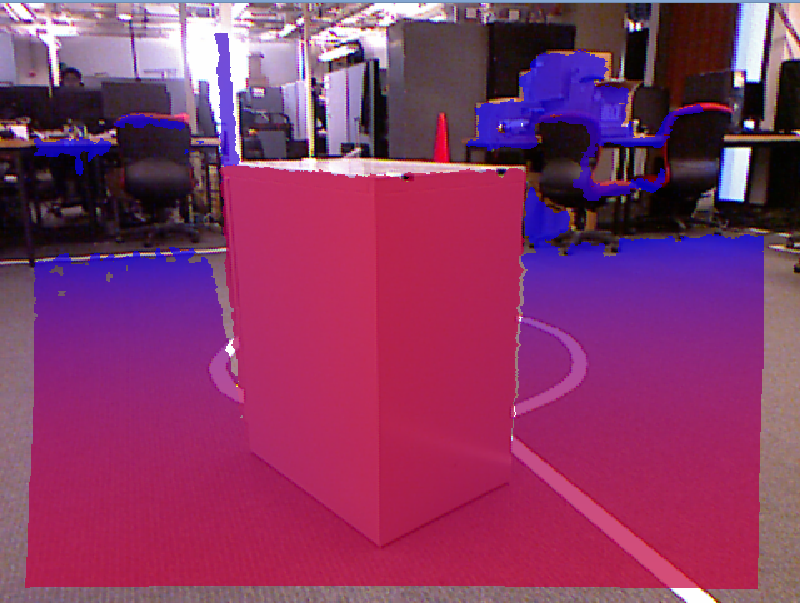
\includegraphics[width=1.0\textwidth]{CabinetDepthOverlay.png}
    \caption{RGB image with depth overlay. Red is closer to the camera, blue is further away. Represents the output of the RGBD Framework}
    \label{fig:rgbdframeworkoutput}
\end{figure}
A crucial component of the pipeline is being able to easily collect RGB-D sensor data from a variety of sources in such a way that the origin of the data is hidden from the remainder of the pipeline. To that end, a highly modular and easily extensible event based framework library was built to seamlessly convert the native data formats and streaming behavior of different sensors. Figure~\ref{fig:rgbdframework} provides an overview of the framework organization. The application code deals directly with four primary classes: RGBDDevice, RGBDFrame, Event Listeners, and FrameLogger. The final output of this framework is a color image and a depth image that are registered in such a way that the pixels have a one-to-one correspondence as shown in Figure~\ref{fig:rgbdframeworkoutput}.
\begin{figure}[ht]
    \centering
    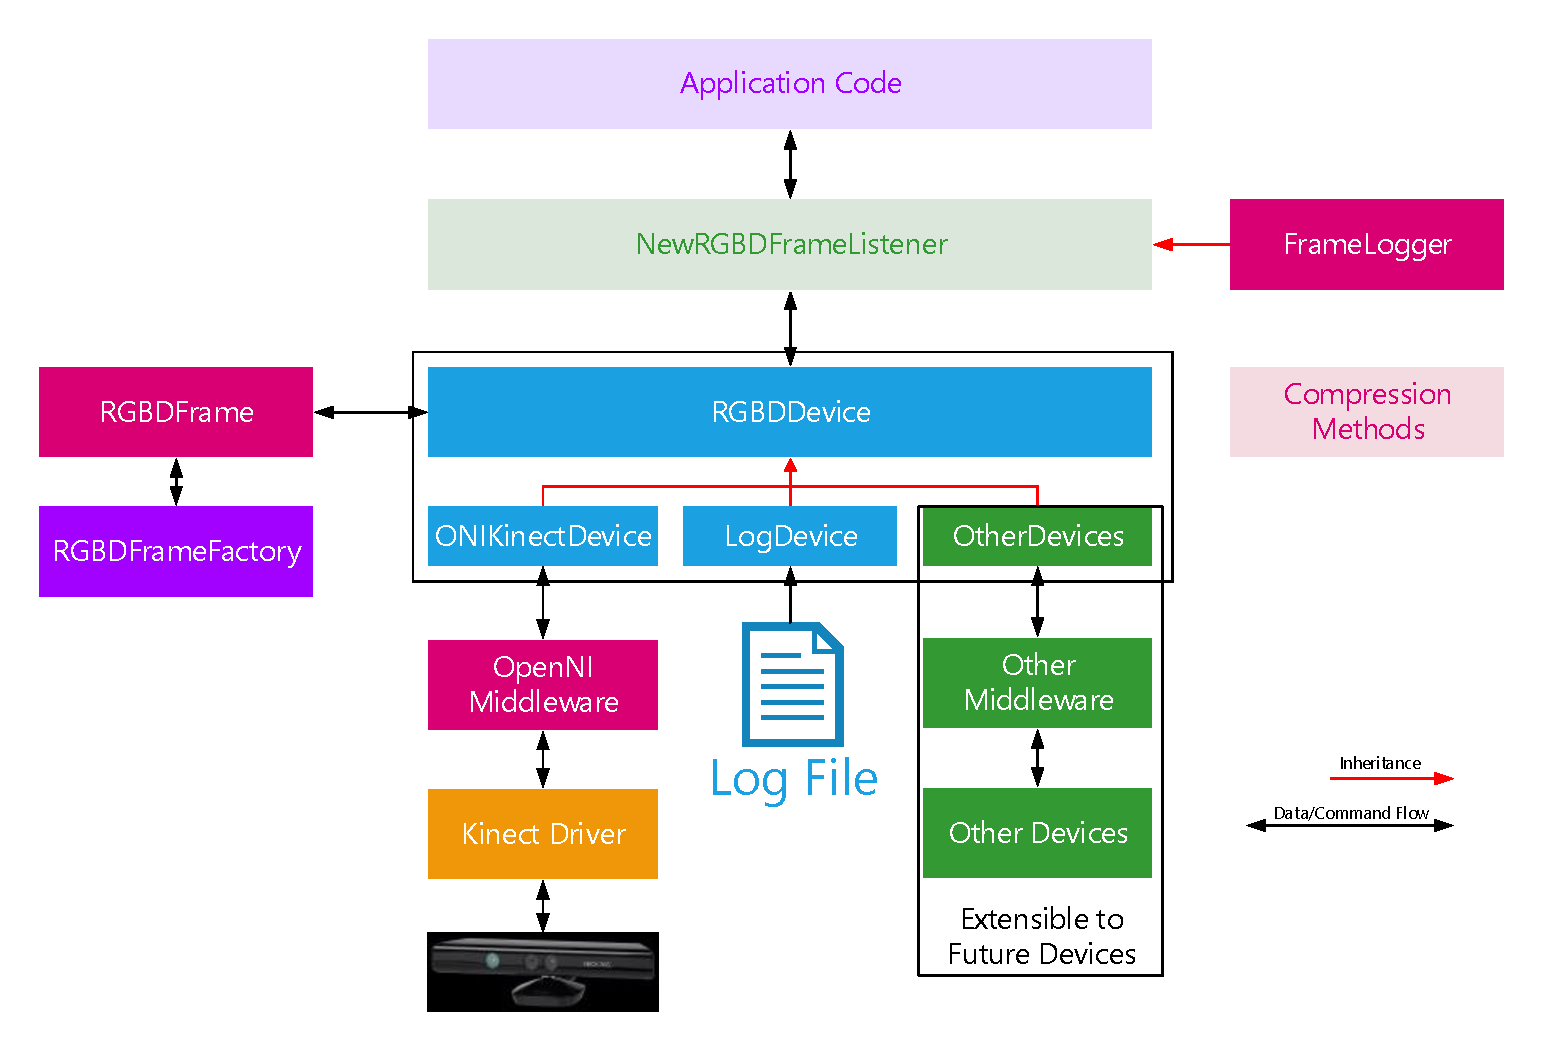
\includegraphics[width=1.0\textwidth]{FrameworkLayout.pdf}
    \caption{RGB-D framework architecture}
    \label{fig:rgbdframework}
\end{figure}
\subsection{RGBDDevice}
The primary interface between the framework and the rest of the application is the abstract class RGBDDevice. RGBDDevice provides an abstract interface including a data stream management API, access to device properties like camera intrinsics and resolution, and event listener registration API. Interfaces for specific devices like the Kinect can be implemented by creating a subclass of RGBDDevice and implementing the abstract methods. The application can then instantiate the desired subclass with device specific initialization parameters and the remainder of the pipeline can be completely agnostic to the underlying nature of the data source, since all RGBDDevices provide the same format RGBDFrame through the same event architecture regardless of the native device formatting. The current framework contains two subclasses: ONIKinectDevice and LogDevice. 
\paragraph{ONIKinectDevice} ONIKinectDevice implements a connection specific to the Microsoft Kinect using OpenNI as middleware. The implementation utilizes OpenNI's event-based interface to receive data from the sensor. Two streams for the color and depth data are created and registered with listeners internal to ONIKinectDevice. When a new depth or color frame is received from OpenNI, the data is copied and repackaged into an RGBDFrame format and a new thread is launched which passes the RGBDFrame to each registered listener. 
\paragraph{LogDevice} LogDevice replays a data log created using the FrameLogger class. Because of the way that the FrameLogger records the data, any device that can be implemented as an RGBDDevice can be recorded and played back using a LogDevice. The framework even allows logging data from a LogDevice. This class allows experiments to be performed very easily on prerecorded data without having to alter the behavior of the pipeline at all.
\subsection{RGBDFrame}
The RGBDFrame is a simple data structure that provides a consistent data formatting for users of the framework. Each frame consists of two managed shared pointers (implemented using boos::shared\_array<T>); one points to the color data and the other points to depth data. Color data is stored in a 24-bit RGB format (1 byte for each component red, green, blue). Depth data is stored in an unsigned 16-bit integer where the least significant bit represents 1mm of resolution (i.e. the value 1024 corresponds to a depth of 1.024m). The frame also has two flags indicating the validity of the depth and color arrays, since not every frame will have both.\par
RGBDFrames are created using a factory design paradigm. The RGBDFrameFactory generates managed pointers which refer to RGBDFrames of a given resolution. Because of the nature of shared pointers, when the last reference to the frames or its component arrays goes out of scope, the frame will delete itself. Because of this, the frames can easily be handed off to the application with no need for the application to be aware of the finer points of the RGBDFramework's memory management scheme. Since roughly 46MB of frame dedicated memory will be allocated every second by the framework, clean, simple memory management is essential.
\subsection{Event Listeners}
The RGBDDevice provides a suite of event listeners that the application code can register listeners for. Four events can be emitted by the RGBDDevice: DeviceConnected, DeviceDisconnected, DeviceMessage, and NewRGBDFrame.
\paragraph{DeviceConnected}
This event is triggered when the underlying device is successfully connected to the RGBDDevice. This usually happens upon success of the RGBDDevice::connect method.
\paragraph{DeviceDisconnected}
This event is triggered when the underlying device is disconnected. This happens either upon calling RGBDDevice::disconnect, or when a fatal communication failure occurs.
\paragraph{DeviceMessage}
This is a special event that allows the device to pass human readable text descriptors to the application for display in the appropriate place. This is useful for debugging or for registering more unique events for a specific device.
\paragraph{NewRGBDFrame}
This event actually transfers the latest RGBDFrame from the sensor to the application. It passes a shared\_ptr to the all registered listeners.
\subsection{FrameLogger}
The FrameLogger class is actually just a special subclass of the NewRGBDFrameListener class. To record the output of any RGBDDevice to a directory, the FrameLogger just needs to be given an output directory using setOutputDirectory. Once that has been done, all that is required to log the output is to call the FrameLogger's startRecording method, which registers the FrameLogger as a NewRGBDFrameListener with the target RGBDDevice. As the logger receives new frames (which can happen in parallel with the primary pipeline), they are tagged with a counter id and saved to the output directory as raw binary files. Some options are also available for data compression.


\section{Filtering and Point Cloud Generation}
\begin{figure}[ht]
    \centering
    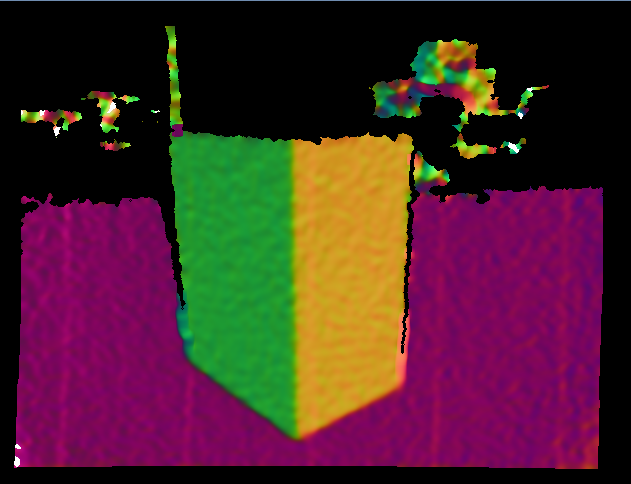
\includegraphics[width=1.0\textwidth]{CabinetNormals.png}
    \caption{Visualization of surface normals, where components of the normal vector are mapped from to rgb. Example of output from preprocessing stage. }
    \label{fig:filteringoutput}
\end{figure}
Once the raw RGB-D frame has been received, it is pushed to GPU memory. This is the only downstream memory transfer that happens during this entire thesis. Once the memory transfer is complete, the next step is to convert the RGBDFrame format into a floating point representation that is easier to manipulate and perform other preprocessing steps like depth filtering and normal estimation. The data is also converted to a structure of arrays format to improve memory coherence. Figure~\ref{fig:preprocessingdiagram} shows the entire preprocessing system's program flow. 
\begin{figure}[hp]
    \centering
    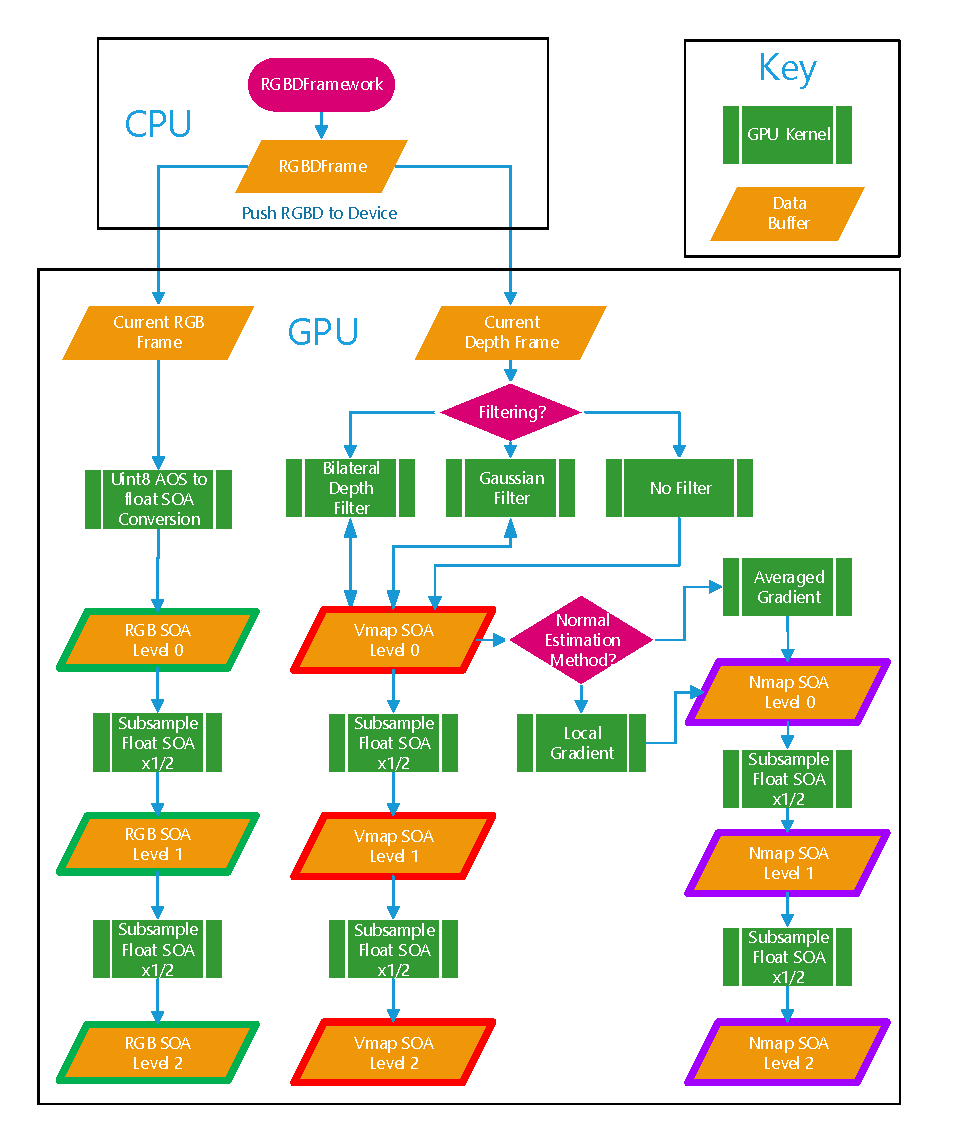
\includegraphics[width=1.0\textwidth]{PreprocessingDiagram.pdf}
    \caption{Preprocessing pipeline diagram.}
    \label{fig:preprocessingdiagram}
\end{figure}
\paragraph{RGB Data Processing} 
The processing for the RGB data is trivial. A kernel converts the 0-255 integer representation of the color data into a 0.0-1.0 floating point representation stored in a structure of arrays (SOA) format for memory coherence. This SOA is then subsampled twice by a factor of two each time, resulting in two additional levels of image resolution. This is useful for later stages in the pipeline that do not require full resolution to function and can therefore be run much faster on the lower resolution image.
\paragraph{Depth Filtering}
The pipeline includes three options for pre-filtering the depth data: no filter, a separable Gaussian filter, and a separable bilateral filter approximation\cite{pham2005separable}. The no filter kernel simply performs the inverse camera projection to convert the depth data into an ordered point cloud stored in the vertex map (VMap) buffer. The formula for this projection is based on the camera intrinsic parameters $\{f_x,f_y,c_x,c_y\}$ and the pixel coordinates $(u,v)$.
$$v_x = (u - c_x) * depth / f_x$$
$$v_y = (v - c_y) * depth / f_y$$
$$v_z = depth$$
Pixels with invalid depth data are stored as NaN to allow easy validation later in the pipeline.\par 
The Gaussian kernel performs the same projection, but also applies a separated implementation of Gaussian filter  $(radius=3 pixels,\sigma=2.0)$ to the depth data before calculating the projection. This helps remove much of the depth quantization and sensor noise that makes normal estimation difficult. However, the Gaussian filter does not preserve edges, so crucial discontinuities in the image are blurred together.\par 
To solve this problem, a bilateral filter is used instead. In addition to the spatial Gaussian term that weights pixels by their screen distance from the center pixel, bilateral filters also apply a Gaussian weight to the difference in intensity. In this way, pixels that have a vastly different depth value will have a lower weight and hard edges can be more easily preserved.\par 
As with the color data, the vertex map is subsampled into a resolution pyramid.
\paragraph{Normal Estimation}
Surface normals are locally estimated for each valid point. Several methods exist for estimating point cloud normals, but the simplest to apply in an ordered image is a gradient based approach. For each point $\vec{p}(x,y)$ Two vectors $\vec{G_x}$ and $\vec{G_y}$ are created from the neighboring points. $$\vec{G_x}(x,y)=\vec{p}(x+1,y)-\vec{p}(x-1,y)$$ $$\vec{G_y}(x,y)=\vec{p}(x,y+1)-\vec{p}(x,y-1)$$
The normalized cross product of these two vectors is then taken to be the point normal. $$\vec{N}(x,y)= \frac{\vec{G_x}(x,y) \times \vec{G_y}(x,y)}{|\vec{G_x}(x,y) \times \vec{G_y}(x,y)|}$$
Since the sign of this normal is ambiguous, all normals are flipped so that they face the viewpoint. The normal faces the viewpoint when the following condition is met: $$\vec{N} \cdot (\vec{p}-\vec{p}_{eye}) < 0$$
Since in the coordinate frame used at this stage has the eye at the origin looking along the $+z$ axis, this condition can be simplified to: $$\vec{N} \cdot \vec{p} < 0$$
If the estimated normal violates this condition, the negative of the normal is stored.\par
While this simple normal estimate works reasonably well, it can be improved by applying a smoothing filter to the gradient images $G_x$ and $G_y$. A separable Gaussian kernel is applied to each gradient image in turn, and then the cross product is performed. Figure~\ref{fig:filtercompare} compares the various combinations of depth filters and normal estimation methods on the normal estimates. Notice how the Gaussian filter fills in the gaps between the cabinet and the floor, but the bilateral filter shows a very clean break. The final pipeline uses both the bilateral filter and the gradient smoothing techniques. And once again, the normals are subsampled and stored in a resolution pyramid.

\begin{figure}[ht]
    \centering
    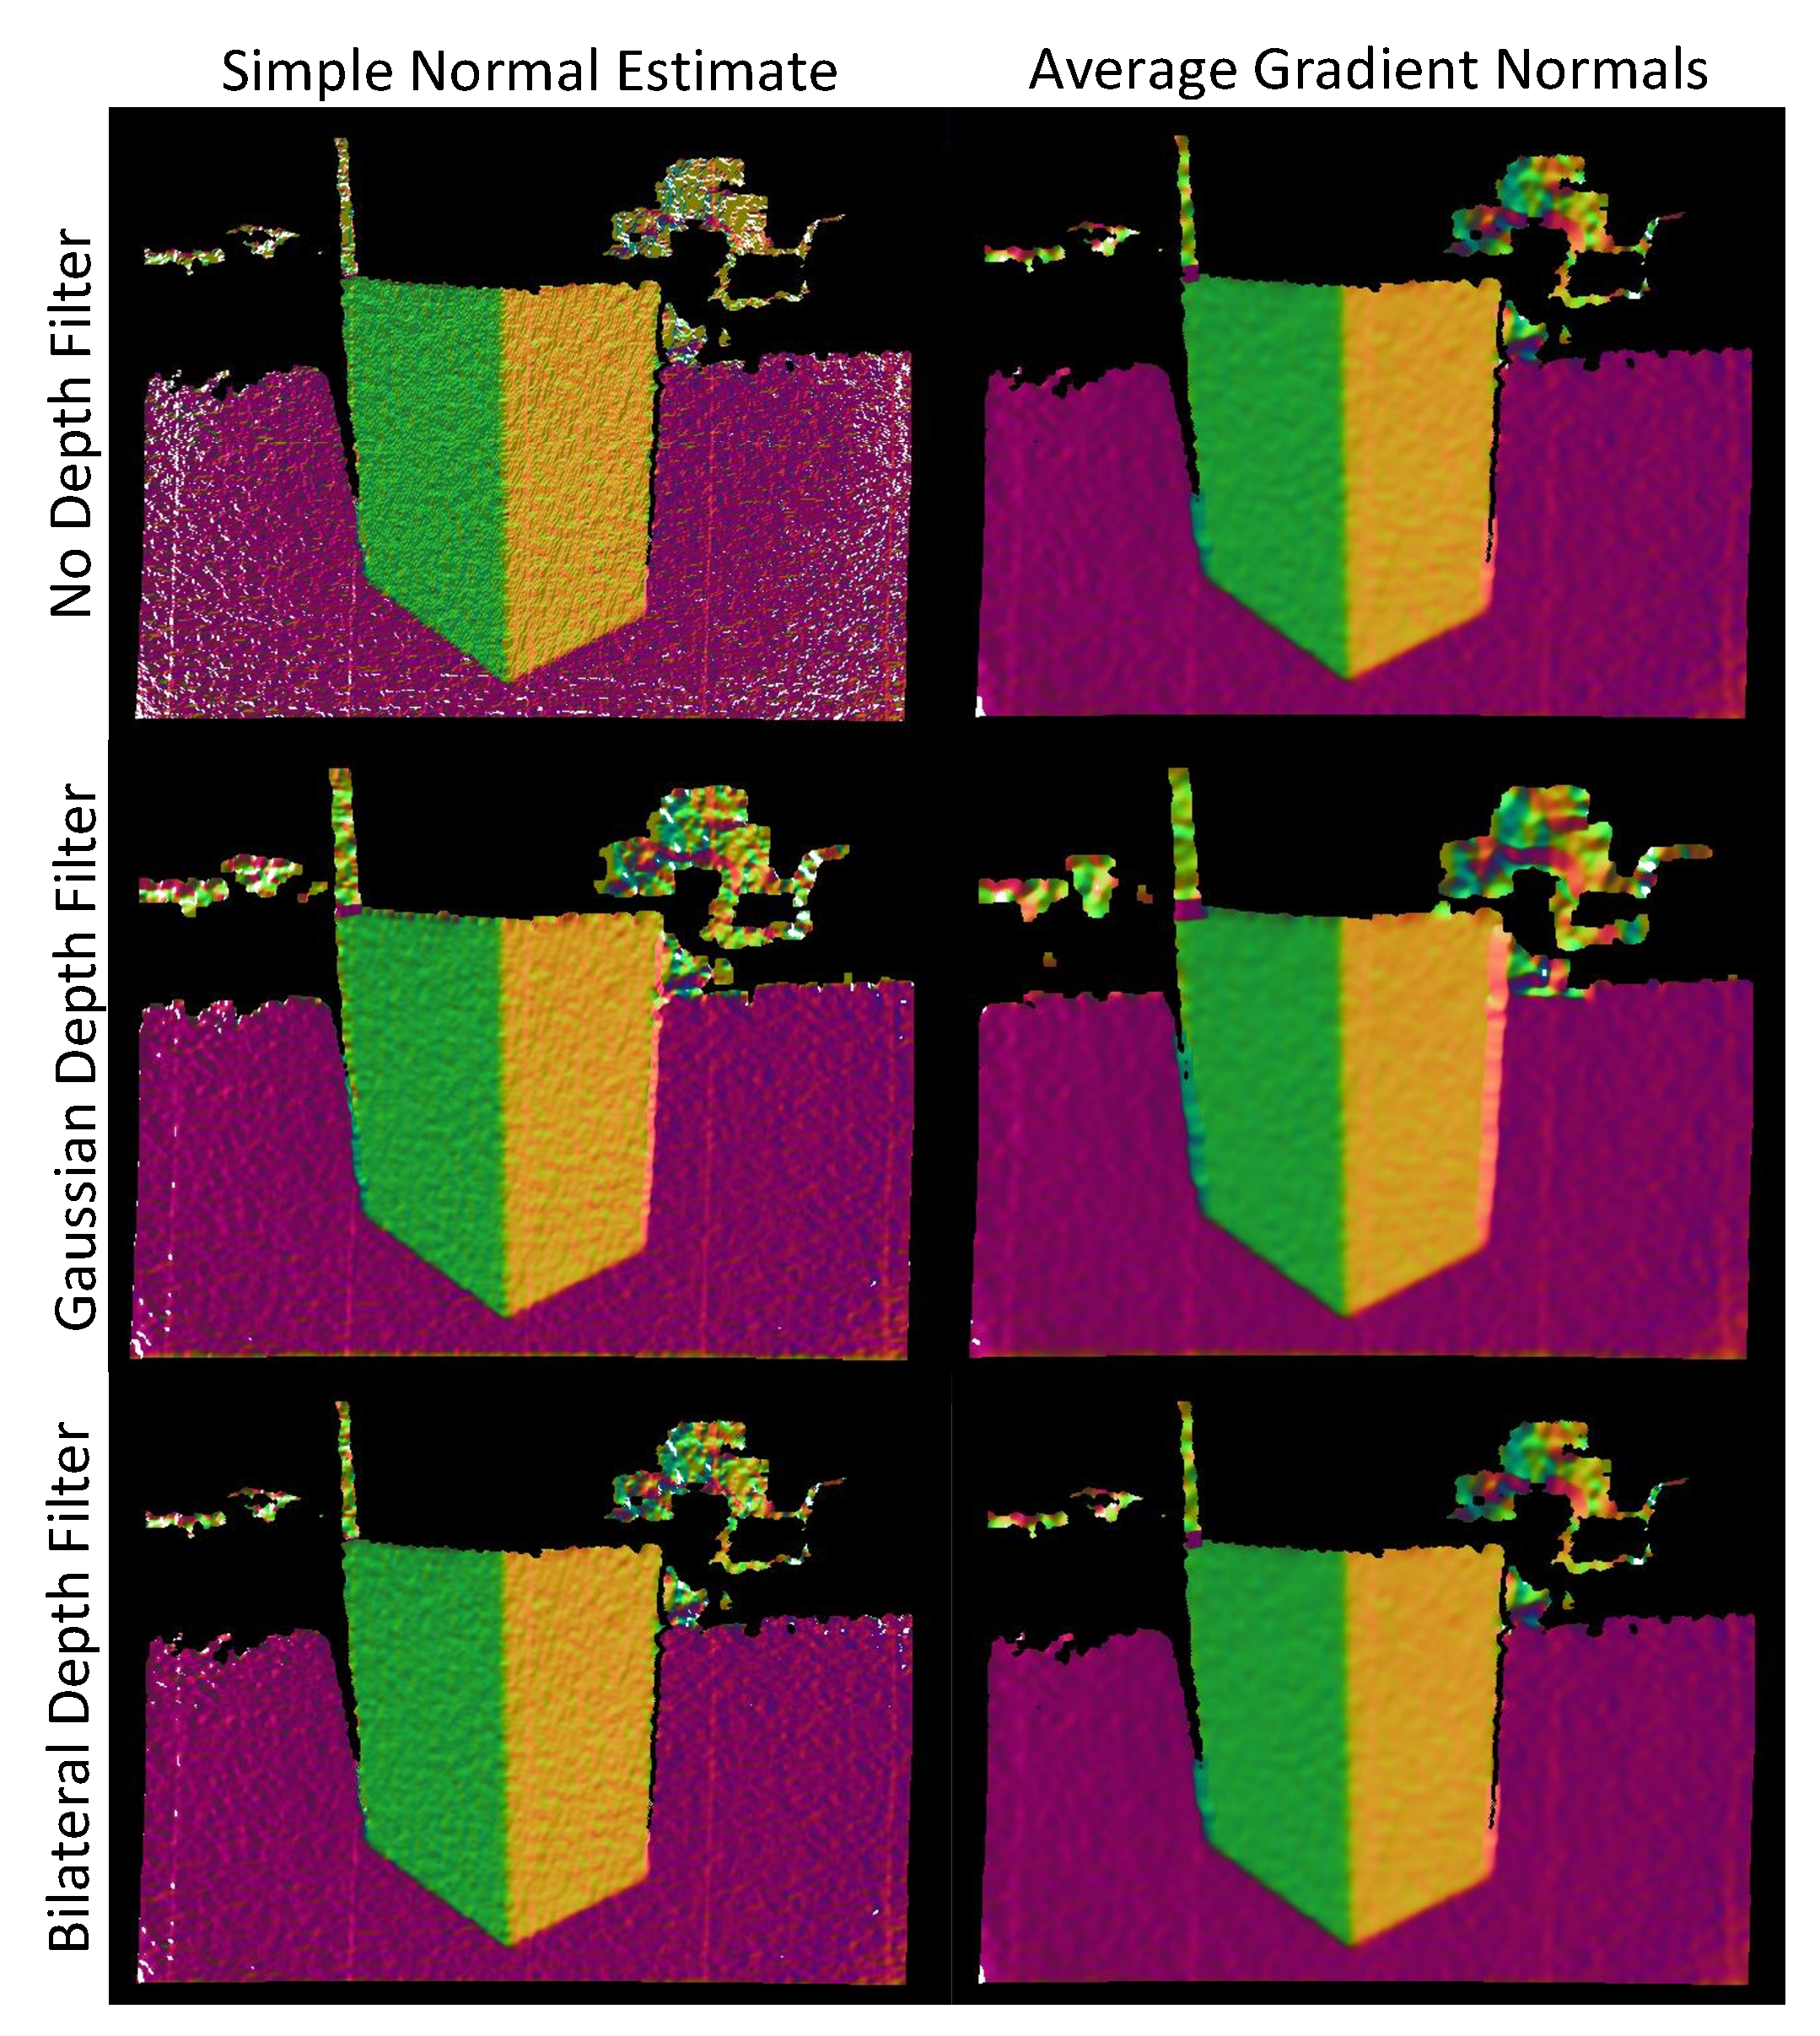
\includegraphics[width=1.0\textwidth]{FilterCompare.pdf}
    \caption{Comparison of the normals estimated using various methods and filters}
    \label{fig:filtercompare}
\end{figure}

\section{Plane Segmentation}
The plane segmentation portion of the pipeline is easily the most complicated (Figure~\ref{fig:segmentationdiagram}). It takes the normals and positions generated by the preprocessing stage as input and outputs a buffer the same size as the original image where each pixel is the index of the detected plane the pixel belongs to, or -1 if the pixel doesn't belong to a plane. The results can be visualized with a random colorization as in Figure~\ref{fig:segmentationoutput}.
\begin{figure}[ht]
    \centering
    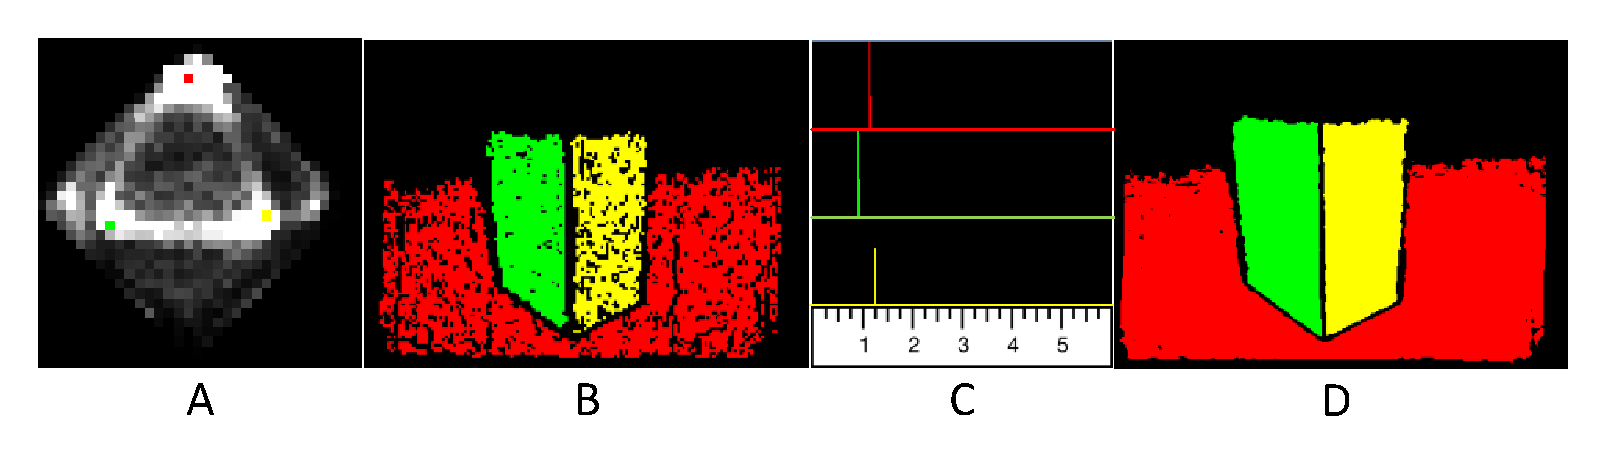
\includegraphics[width=1.0\textwidth]{SegmentationStages.pdf}
    \caption{Buffers from various stages of the segmentation pipeline. A) The 2D normal histogram with 3 identified peaks. B) Normal Segmented Image. C) Distance histograms for refinement. D) Final Segmentation.}
    \label{fig:segmentationstages}
\end{figure}

The overall approach to image segmentation is inspired by Holz \textit{et al.}\cite{holz2012real}. The initial step is to detect clusters of similarly oriented surface normals. A two-dimensional histogram of the normals is created, and a collection of dominant peaks is detected (Figure~\ref{fig:segmentationstages}A). Once these peaks have been detected, the initial segmentation pass segments all normals that are very close to the peak (Figure~\ref{fig:segmentationstages}B). Using only the points from the detected segments, a distance histogram is computed for each peak, where the distance value of each point is computed using the dot product of the peak normal and the point's position in camera space(Figure~\ref{fig:segmentationstages}C). In addition to refining the segmentation in distance space, some basic statistics about the detected planes are collected. Because the original normal estimate from the original histogram can be very coarse, the plane stats are used to realign the normal peaks more accurately. The entire inner loop is run again with the accurate normals, yielding cleaner results in complex scenes. After the second run through, the planes are finalized and the final segmentation buffer is updated (Figure~\ref{fig:segmentationstages}D). Optionally, this entire process can be run multiple times excluding previously segmented pixels to detect planes that were previously obscured by larger noisy peaks.

\begin{figure}[hp]
    \centering
    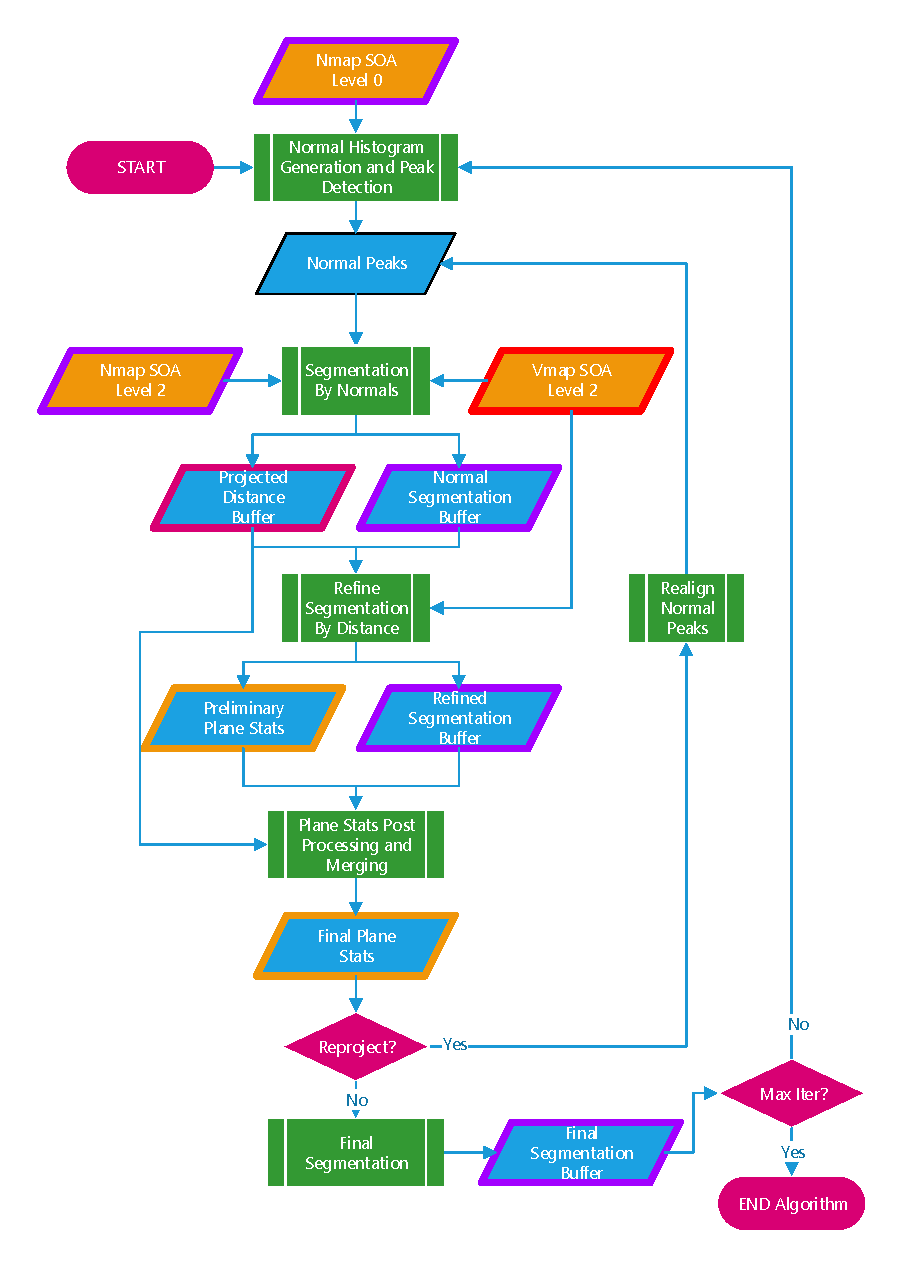
\includegraphics[width=1.0\textwidth]{SegmentationProcess.pdf}
    \caption{Plane segmentation pipeline diagram.}
    \label{fig:segmentationdiagram}
\end{figure}

\begin{figure}[ht]
    \centering
    
\includegraphics[width=1.0\textwidth]{CabinetPlanes.png}
    \caption{Random colorization of detected planes. Example of output from segmentation stage.}
    \label{fig:segmentationoutput}
\end{figure}

\subsection{Normal Histogram Generation and Peak Detection}
Holz\cite{holz2012real} used a 3D voxel grid to discretize normal space, although they also experimented with a two-dimensional $(\phi,\theta)$ space. They then merged clusters with their neighbors to come up with their final segmentation. Unfortunately, this approach does not map well to the GPU. As an alternative, I created a very simple index mapping $[n_x,n_y,n_z] \to [\frac{\cos^{-1}(n_x)}{\pi}*numBinsX,\frac{\cos^{-1}(n_y)}{\pi}*numBinsY]$ where $numBinsX$ and $numBinsY$ are the resolution of the histogram. Instead of doing sophisticated clustering, I do simple iterative global maximum detection using a high speed parallel reduction algorithm. After each peak is detected, a region of histogram space is cleared to avoid just off max peaks from being recorded. This iteration continues until the maximum number of peaks have been detected or no peak is above the minimum threshold count. Each detected peak index is then reverse mapped to a peak normal vector. To improve accuracy slightly, the normal is computed using an average of the neighboring normals weighted by the histogram count.\par
One important thing to note about histogram generation in parallel is the runtime performance is heavily data dependent. If two threads running concurrently try to increment the same histogram bin, a race condition occurs and the result is corrupted. This requires using atomic operations to serialize these additions. As a result, the worst case scenario is a single noiseless plane that fills the entire image. By contrast, calculating the histogram on the CPU would be constant runtime. In my experiments, the CPU runtime plus memory transfers took longer than most GPU scenarios, but the ultimately it is an engineering tradeoff. Alternatively, the resolution of the histogram can be increased, which statistically decreases the number of write conflicts. However, this makes peak detection slightly more complicated to implement efficiently. Again, tradeoffs to be considered another time.
\subsection{Segmentation By Normals}
This step is fairly self explanatory. Using the peaks detected in the previous step, if the normal of a point deviates from a peak normal by less than 5 degrees, the pixel is assigned to that peak. This step also computes the projected distance of the point for use in the next step. The distance calculation is derived from the plane equation: $$a*x+b*y+c*z=dist$$
Using the corresponding peak normal as the constant parameters $[a,b,c]$ and the point's camera space position as the $[x,y,z]$ values, $dist$ is simply the dot product $$dist=\vec{N}_{peak} \cdot \vec{p}_{cam}$$

\subsection{Refine Segmentation by Distance}
This stage serves two functions. First, multiple planes can have the same normal but different distance offsets. A door recessed into a wall is a very common example in human environments. Using the projected distance along the normal to a parallel plane passing the origin and creating a histogram of these distances (Figure~\ref{fig:segmentationstages}C), each plane should stand out as a unique peak. However, if the plane normal estimate from the peak detection step was too far off from the ground truth plane normal then these peaks will be smeared and difficult to detect. This is the primary reason that the inner loop is run twice, once to have a shot at detecting some portion of a plane to get a truer normal, and a second run with the true normal to find the actual planes. Without this step, large planes were often broken into several smaller strips or planes that were not offset by much were merged incorrectly.\par 
Once the distance peaks are located, the previous segmentation is refined with only points corresponding to distance peaks remaining. For efficiency, the same kernel that updates the segmenation buffer also collects the first pass plane statistics. Each plane's pixel count, centroid, and scatter matrix are computed in this stage, though the values are just stored as accumulated sums. The data collected here will be processed in the next stage.
\subsection{Plane Statistics Processing and Plane Merging}
This stage calculates various defining features of the planes. The statistics collected were inspired by Biswas\textit{et al.} work on a RANSAC based plane filtering algorithm\cite{biswas2012planar}. The plane centroid is computed as: $$\bar{p}=\frac{1}{n}*\sum_{p_i \in P}{p_i}$$ where $n$ is the number of points in the planar segment. To compute the plane normal and tangent, the scatter matrix of the plane could be computed as: $$S = \sum_{p_i \in P}(p_i-\bar{p})(p_i-\bar{p})^T$$.
However, merging the planes becomes much simpler if the matrix can be decoupled from the centroid\cite{biswas2012planar}. So let 
$$S_1 = \frac{1}{n}\begin{bmatrix}
  \sum{x_i x_i} & \sum{x_i y_i} & \sum{x_i z_i} \\
  \sum{y_i x_i} & \sum{y_i y_i} & \sum{y_i z_i} \\
  \sum{z_i x_i} & \sum{z_i y_i} & \sum{z_i z_i}
 \end{bmatrix}$$
and
 $$S_2 = \begin{bmatrix}
  \bar{x}\bar{x} & \bar{x}\bar{y} & \bar{x}\bar{z} \\
  \bar{y}\bar{x} & \bar{y}\bar{y} & \bar{y}\bar{z} \\
  \bar{z}\bar{x} & \bar{z}\bar{y} & \bar{z}\bar{z}
 \end{bmatrix}$$
then the matrix
 $$S'=S_1-S_2$$
is a normalized representation of the scatter matrix that can be used to compute the plane normal and tangent. Planes can then be conditionally merged by the procedure outlined by Biswas\cite{biswas2012planar}. 
The eigenvector corresponding to the smallest eigenvalue is taken to be the plane normal, while one of the other eigenvectors is chosen to be the tangent vector. The tangent vector is chosen such that all planes are oriented in roughly the same way in screen space, with the tangent vector roughly corresponding to the $+y$ axis.
\subsection{Final Segmentation}
Once all the planes have been finalized, all points in the image are considered and evaluated to find the best fit. Points are assigned to planes using the following minimization procedure:
$$PlaneId_i = \operatorname{arg\,min}_{plane} [ p_i \cdot \vec{N}_{plane} ]$$ s.t. $$|\vec{N}_i \cdot \vec{N}_{plane}| > angleThreshold$$ and $$p_i \cdot \vec{N}_{plane} < distThreshold$$
The angle threshold can generally be set very wide, as much as $cos(\pi*15/180)$, since the dominating factor will be distance to the plane.
\section{Planar Mesh Generation}
\begin{figure}[ht]
    \centering
    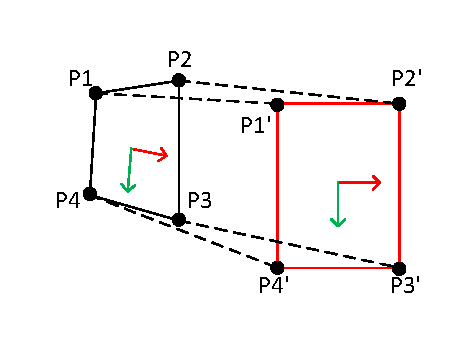
\includegraphics[width=0.5\textwidth]{ProjectiveTransform.pdf}
    \caption{Projective transform example}
    \label{fig:projectivetransform}
\end{figure}

\begin{figure}[ht]
    \centering
    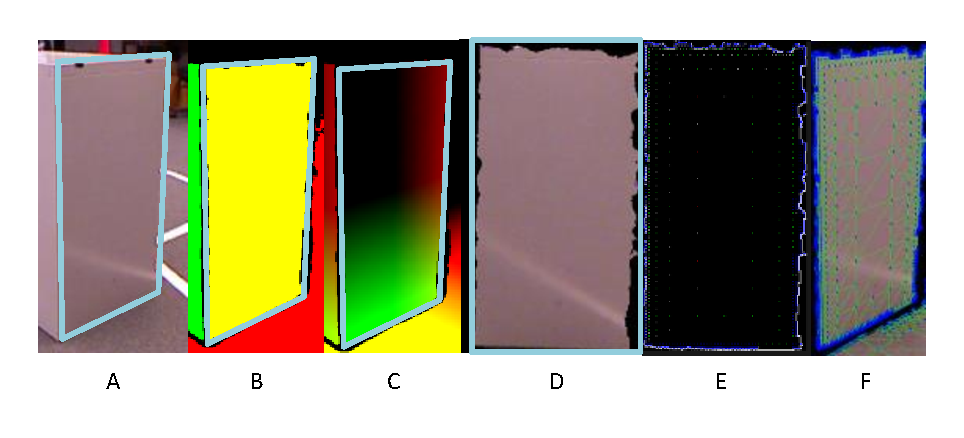
\includegraphics[width=1.0\textwidth]{QuadtreeDecimation.pdf}
    \caption{Stages of QuadTree Generation: A) Original RGB Image with AABB imposed, B) Plane Segmentation with AABB imposed, C) $(S_x,S_y)$ coordinate system visualized. Green intensity corresponds to $+S_y$ value and red intensity to $+S_x$, D) Flat projected RGB texture with projected AABB, E) QuadTree verticies visualized in flat projection space, F) Final QuadTree mesh visualized with virtual camera}
    \label{fig:quadtreestages}
\end{figure}

Once the individual planes have been segmented, each plane is reduced using a parallelized version of QuadTree Based triangulation\cite{planesegmentationQTB}. The first step is to calculate the inverse projection of the plane onto a flat surface that is uniformly scaled in X and Y as in Figure~\ref{fig:projectivetransform}.
The first step is to compute an axis-aligned bounding box (AABB) for each plane in the 2D coordinate frame defined by the plane's tangent and bitangent vectors $\vec{T}$ and $\vec{B}$. The plane's normal and tangent vectors are stored in the plane statistics, and the bitangent can be computed from the cross product $\vec{B}=\vec{N} \times \vec{T}$.\par
The position of a camera space point $p$ in this coordinate system $(S_x,S_y)$ can be computed as: $$S_x=\vec{B} \cdot (p - \bar{p})$$ $$S_y=\vec{T} \cdot (p - \bar{p})$$
Using a parallel reduction algorithm, the minimum and maximum values of $S_x$ and $S_y$ for each plane are computed. This provides an AABB in meters for each segment (Figure~\ref{fig:quadtreestages}C). To compute the projection matrix from camera space to flat space, the screen space coordinate pairs $(u_{source,i},v_{source,i})$ are computed for each corner using the bounding box and camera intrinsics: 
$$p_1 = (AABB_{x,min} * \vec{B})+(AABB_{y,min} * \vec{T})+\bar{p}$$
$$p_2 = (AABB_{x,max} * \vec{B})+(AABB_{y,min} * \vec{T})+\bar{p}$$
$$p_3 = (AABB_{x,max} * \vec{B})+(AABB_{y,max} * \vec{T})+\bar{p}$$
$$p_4 = (AABB_{x,min} * \vec{B})+(AABB_{y,max} * \vec{T})+\bar{p}$$
$$u_{source,i} = \frac{p_{i,x}*fx}{p_{i,z}} + cx$$
$$v_{source,i} = \frac{p_{i,y}*fy}{p_{i,z}} + cy$$
The resolution of the final image is selected such that the final projected image will be less than 1024x1024 and resolution given in pixels/meter is a power of 2. This makes textures from various meshes much easier to compare directly by simple up-sampling or down-sampling. Once a resolution has been selected, the destination width and height $w_d$ and $h_d$ in pixels can be computed directly from the AABB dimensions and the pixels/m resolution: 
$$w_d=resolution_{px/m} * {AABB_{x,max}-AABB_{x,min}}$$
$$h_d=resolution_{py/m} * {AABB_{y,max}-AABB_{y,min}}$$
Now the transform matrix $T$ can be calculated by the following procedure. Let:
$$\begin{bmatrix}
  u_{s,1} & u_{s,2} & u_{s,3} \\
  v_{s,1} & v_{s,2} & v_{s,3} \\
  1 & 1 & 1 
 \end{bmatrix} * \vec{x} = \begin{bmatrix}
  u_{s,4} \\
  v_{s,4} \\
  1
 \end{bmatrix}$$
Solve for $\vec{x}= A^{-1}*b$ and then multiply through the original matrix by $\vec{x}$ such that:
$$A = \begin{bmatrix}
  x_1*u_{s,1} & x_1*u_{s,2} & x_1*u_{s,3} \\
  x_2*v_{s,1} & x_2*v_{s,2} & x_2*v_{s,3} \\
  x_3 & x_3 & x_3 
 \end{bmatrix}$$
This matrix represents a transformation from the source coordinate system to an orthogonal basis vector set. Next the transform from the destination coordinate frame to the basis vector set is computed in a similar fashion.
$$\begin{bmatrix}
  0 & w_d & w_d \\
  0 & 0 & h_d \\
  1 & 1 & 1 
 \end{bmatrix} * \vec{x} = \begin{bmatrix}
  0 \\
  h_d \\
  1
 \end{bmatrix}$$
Solve for $\vec{x}= A^{-1}*b$ and then multiply through the original matrix by $\vec{x}$ such that:
$$A = \begin{bmatrix}
  0 & x_1*w_d & x_1*w_d \\
  0 & 0 & x_2*h_d \\
  x_3 & x_3 & x_3 
 \end{bmatrix}$$
Finally, the total transform can be computed $$T=A*B_{-1}$$
Multiplying this transform by a pixel location in the destination image will compute the corresponding pixel location in the original RGB image after dehomogenization, allowing for a very simple projection algorithm implementation that is parallel by destination pixel.
$$s = T*[d_x,d_y,1]^T$$
$$x_{source} = s_x/s_z$$
$$y_{source} = s_y/s_z$$

Now that the texture has been projected to flat space (Figure~\ref{fig:quadtreestages}D), the parallel QuadTree reduction algorithm is run. To simplify the problem, the QuadTree is aligned to the pixel grid of the flat image. This allows for coherent memory access, simple indexing, and very fast parallel decimation. A degree buffer is initialized with -1 for invalid pixels and 0 for pixels that are a part of the plane segment (Figure~\ref{fig:decimation}). The degree number of a pixel indicates size of the quad with the upper left corner at that pixel. Algorithm~\ref{alg:quadtree} shows how the QuadTree decimation works. As an optimization, the kernel was divided into two phases, one for reduction steps 1 through 16, and another for 32 through 256. This breakdown allows the entire process to be done in 16x16 blocks of shared memory, greatly accelerating the process.\par
Once the degree buffer has been filled, the vertices are stream compacted and a triangle index buffer is populated linking the compacted vertices. Each vertex is a 4 float vector containing the plane coordinate system $(S_x,S_y)$ coordinates of the point and the $(u,v)$ texture mapping coordinates. Each quad consists of two triangles using CCW winding order, the OpenGL default. These buffers can be directly drawn to the screen using OpenGL triangle elements (Figure~\ref{fig:meshoutput}).\par
Each mesh is then pulled from the GPU along with their generated textures. The transformation matrix $H_{plane}$ from plane space to camera space is also generated at this point so that the plane can be drawn in the correct location on the screen. 
$$H_{trans} = \begin{bmatrix}
  1 & 0 & 0 & \bar{p}_x \\
  0 & 1 & 0 & \bar{p}_y \\
  0 & 0 & 1 & \bar{p}_z \\
  0 & 0 & 0 & 1
 \end{bmatrix}$$
 $$H_{rotate} = \begin{bmatrix}
  \vec{B} & \vec{T} & \vec{N} & 0 \\
  0 & 0 & 0 & 1
 \end{bmatrix}$$
$$H_{plane} = H_{trans}*H_{rotate}$$
\begin{algorithm}[H]
\label{alg:quadtree}
 \singlespacing
 \KwData{Degree array D with 0 indicating valid pixels, -1 otherwise}
 \KwResult{Degree array D with QuadTree decimation results}
 \ForEach{pixel (x,y) in parallel}{
 
	 \tcc{First step is special case}
	 \If{D[x][y] == 0 and D[x+1][y] == 0 and D[x][y+1] == 0 and D[x+1][y+1] == 0}{
		 D[x][y] = 1\;
	 }
	 
	 \tcc{Quadtree decimation loop}
	 step = 1\;
	 \While{step $<$ 256}{
	 	\tcc{If pixel correctly aligned for this step}
	 	\If{x mod (2*step) == 0 and y mod (2*step) == 0}{
			\tcc{If the four corners of this quad all have the correct degree}
	 		\If{D[x][y] == step and D[x+1][y] == step and D[x][y+1] == step and D[x+1][y+1] == step}{
	 			\tcc{Increase the degree of the upper left corner}
	 			D[x][y] *= 2\;
	 			\tcc{Clear the other three mid points}
	 			D[x+1][y] = -1\;
	 			D[x][y+1] = -1\;
	 			D[x+1][y+1] = -1\;
	 		}
	 	}
	 	
	 	step $<<$= 1\;
	 	syncthreads()\;
	 }
	 
	 \tcc{Patch holes.}
	 \If{D[x][y] $>$ 0}{
	 	\If{D[x+D[x][y]][y] $<$ 0}{
	 		D[x+D[x][y]][y] = 0\;
	 	}
	 	\If{D[x][y+D[x][y]] $<$ 0}{
	 		D[x][y+D[x][y]] = 0\;
	 	}
	 	\If{D[x+D[x][y]][y+D[x][y]] $<$ 0}{
	 		D[x+D[x][y]][y+D[x][y]] = 0\;
	 	}
	 }
 }
 
 \caption{QuadTree Decimation}
\end{algorithm}


\begin{figure}[ht]
    \centering
    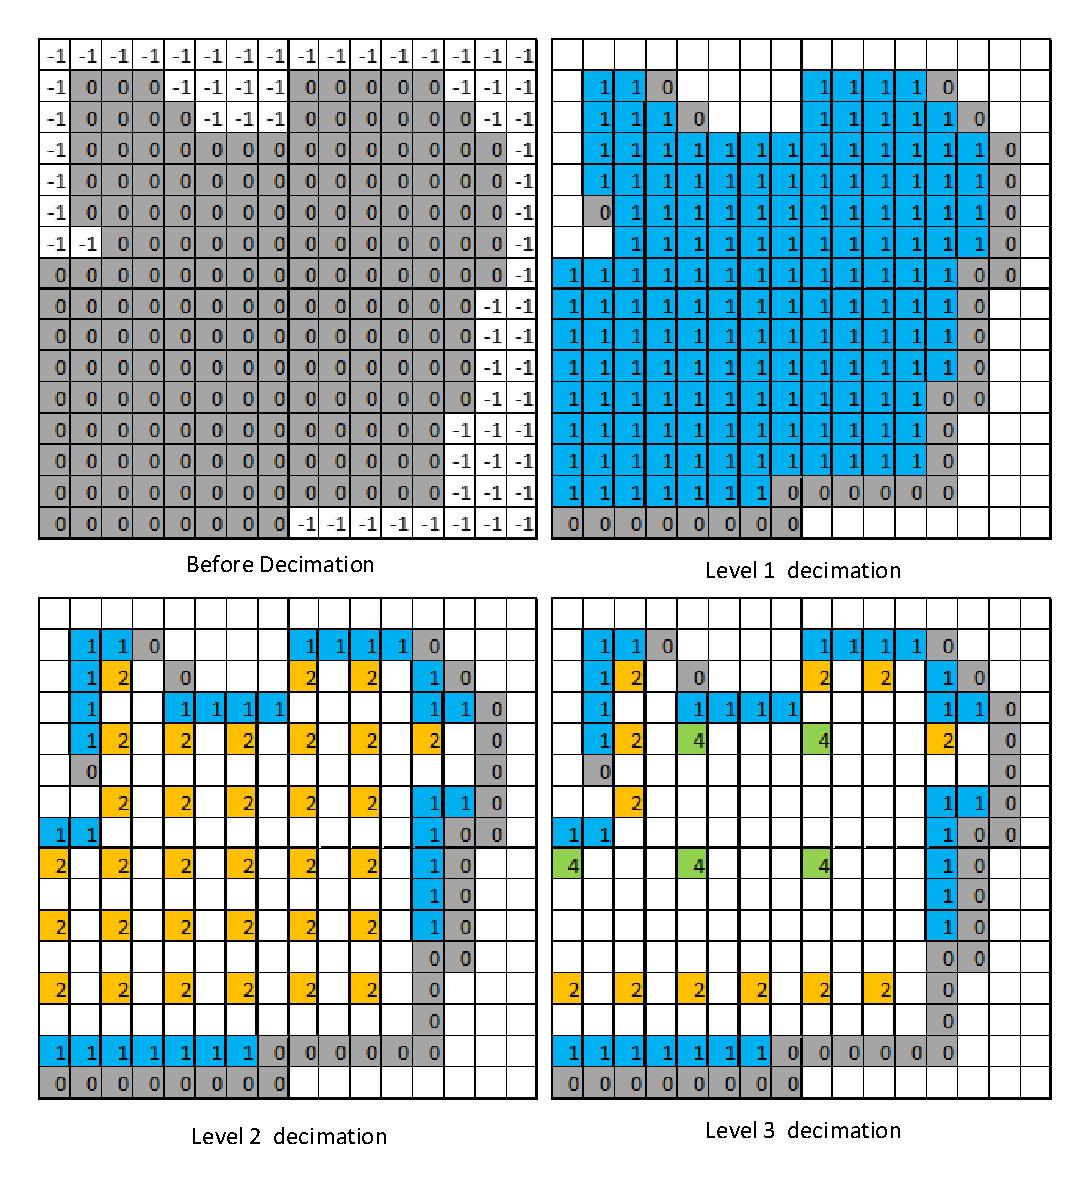
\includegraphics[width=1.0\textwidth]{SampleDecimation.pdf}
    \caption{Example contents of the QuadTree degree buffer at various stages of decimation}
    \label{fig:decimation}
\end{figure}



\begin{figure}[ht]
    \centering
    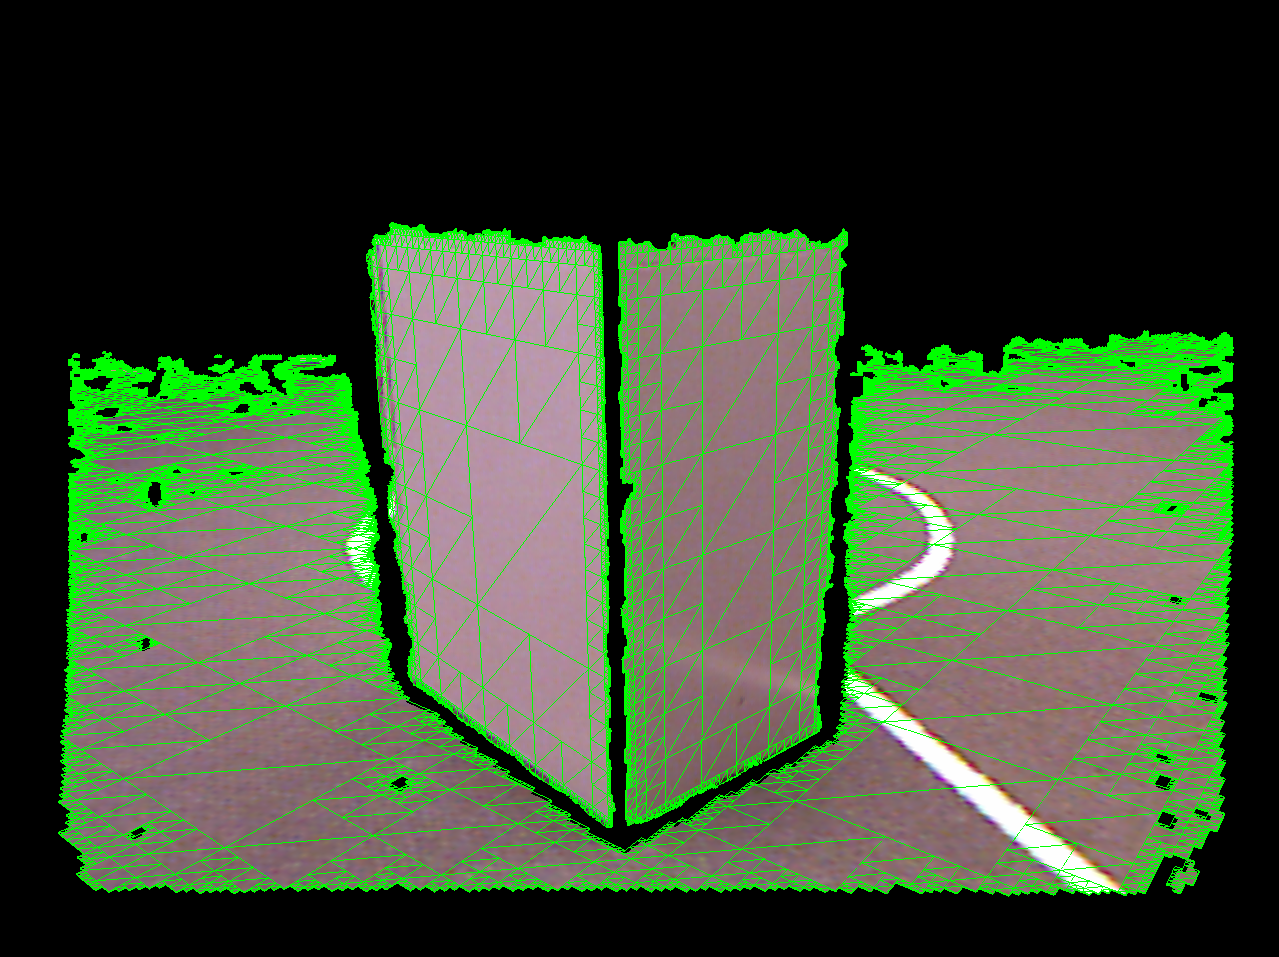
\includegraphics[width=1.0\textwidth]{CabinetMesh.png}
    \caption{Wireframe visualization of the textured mesh. Rendered using the intrinsic parameters of the original camera for direct comparison. Example of output from mesh generation stage.}
    \label{fig:meshoutput}
\end{figure}

